\documentclass[12pt]{article}
\usepackage{amssymb}
\usepackage{amsthm}
\usepackage{dsfont}
\usepackage{amsmath}
\usepackage[latin1]{inputenc}
\usepackage[english]{babel}
\usepackage{graphicx}
\usepackage{bbm}
\usepackage{tikz}
\usepackage{color} 
%\usepackage{nath}
%\delimgrowth=1

\usepackage[margin=1in,footskip=0.25in]{geometry}
\linespread{1.3}

\usepackage{verbatim}
\usepackage{enumitem}

\newtheorem{theorem}{Theorem}%[section]
\newtheorem{lemma}[theorem]{Lemma}
\newtheorem{proposition}[theorem]{Proposition}
\newtheorem{corollary}[theorem]{Corollary}
\newtheorem{question}{Open question}
\newtheorem{defi}[theorem]{Definition}
\theoremstyle{plain}
\newtheorem{assumption}{Assumption}

\theoremstyle{remark}
\newtheorem{remark}{Remark}
\newtheorem{example}{\it Example\/}

\theoremstyle{definition}
\newtheorem{exercise}{Exercise}
\newtheorem{problem}{Problem}

\def\RRn{\mathbb{R}^n}
\def\RR{\mathbb{R}}
\def\RRN{\mathbb{R}^N}
\def\ZZ{\mathbb{Z}}
\def\ZZN{\mathbb{Z}^N}
\def\RRnm{\mathbb{R}^{n \times m}}
\def\RRmn{\mathbb{R}^{m \times n}}

\def\dd{\, \mathrm{d}}

\def\grad{\nabla}
\def\weakConv{\rightharpoonup}
\def\LL{\mathrm{L}}
\def\WW{\mathrm{W}}
\def\naturals{\mathbb{N}}

\def\intRRn{\int_{\RRn}}

\def\calM{\mathcal{M}}
\def\calE{\mathcal{E}_p}
\def\calC{\mathcal{C}}

\def\dist{\text{dist}}
\def\supp{\text{supp}}
\def\indyk{\mathds{1}}

\def\intOmega{\int_{\Omega}}
\def\intRRnm{\int_{\RRnm}}

\def\PP{\mathrm{P}}

\def\Ccinfty{C_c^{\infty}}

\DeclareMathOperator{\im}{Im}
\DeclareMathOperator{\id}{Id}
\renewcommand{\phi}{\varphi}
\renewcommand{\epsilon}{\varepsilon}
\renewcommand{\geq}{\geqslant}
\renewcommand{\leq}{\leqslant}
\renewcommand{\div}{\text{div}}

\newcommand{\measurerestr}{%
  \,\raisebox{-.127ex}{\reflectbox{\rotatebox[origin=br]{-90}{$\lnot$}}}\,%
}

\def\Xint#1{\mathchoice
{\XXint\displaystyle\textstyle{#1}}%
{\XXint\textstyle\scriptstyle{#1}}%
{\XXint\scriptstyle\scriptscriptstyle{#1}}%
{\XXint\scriptscriptstyle\scriptscriptstyle{#1}}%
\!\int}
\def\XXint#1#2#3{{\setbox0=\hbox{$#1{#2#3}{\int}$ }
\vcenter{\hbox{$#2#3$ }}\kern-.6\wd0}}
\def\ddashint{\Xint=}
\def\dashint{\Xint-}

\renewcommand{\phi}{\varphi}
\renewcommand{\epsilon}{\varepsilon}
\renewcommand{\geq}{\geqslant}
\renewcommand{\leq}{\leqslant}

\def\RRn{\mathbb{R}^n}
\def\RR{\mathbb{R}}
\def\RRN{\mathbb{R}^N}
\def\ZZ{\mathbb{Z}}
\def\ZZN{\mathbb{Z}^N}
\def\multiindices{\mathbb{Z}^N_+}
\def\RRnm{\mathbb{R}^{n \times m}}
\def\RRmn{\mathbb{R}^{m \times n}}
\def\naturals{\mathbb{N}}

\def\Ccinfty{C_c^{\infty}}

\def\dd{\, \mathrm{d}}
\def\grad{\nabla}
\def\weakConv{\rightharpoonup}

\def\intRRn{\int_{\RRn}}
\def\intOmega{\int_{\Omega}}
\def\intRRnm{\int_{\RRnm}}
\def\intRRN{\int_{\RRN}}

\def\RRNn{\RR^{N \times n}}

\def\CC{\mathrm{C}}

\def\RRn{\RR^n}
\def\RRm{\RR^m}


\usetikzlibrary{shapes, arrows, calc, arrows.meta, fit, positioning}  
\tikzset{  
    -Latex,auto,node distance =1.5 cm and 1.3 cm, thick,
    state/.style ={ellipse, draw, minimum width = 0.9 cm}, 
    point/.style = {circle, draw, inner sep=0.18cm, fill, node contents={}},  
    bidirected/.style={Latex-Latex}, 
    el/.style = {inner sep=2.5pt, align=right, sloped}  
}  


\def\hint{\noindent \textbf{Hint: }}
\begin{document}

\begin{center}
\begin{Large}
\textbf{LN fee bounds}

\end{Large}
\text{sketch}
\end{center}

\begin{itemize}
  \item B - price of 1 on-chain transaction
  \item r - market interest rate - effective internal rate of return with continuous compounding
  \item $c(B,\lambda,r)$ - amount in a single transaction  \textbf{[add reference for the equation]}
  \item $\lambda$ - transaction frequency
  \item $\alpha$ - average lifetime of a channel
  \item $3(\frac{2B\lambda}{r})^{1/3}$ - expected cost of a bidirectional channel (opening, reopening, maintaining)
  \item $\sqrt{\frac{2B\lambda c}{r}}$ - expected cost of an unidirectional channel
  \item $N(\lambda, t)$ - Poisson i.i.d random variable for count of transactions in terms of $\lambda$ in time period $(0,t]$ 
  \item p - the fixed transaction fee for each payment c. It could be changed into a function of c
\end{itemize}

\section{Cycle of 6}
Let there be an unidirectional channel from Alice to Bob, and bidirectional channel between Bob and Donna, Donna and Frank, Frank and Emily, Emily and Charlie, and Charlie and Alice, creating a cycle with 1 unidirectional channel and 5 bidirectional channels. 
\\ The furthest node from Alice is Frank, and Alice wants to send a fixed payment to Frank. We analyze the difference between 2 routes and Alice creating a directional channel to Frank. 
\\ If no one act as an intermediate node, then ithout Alice has to create a direct channel with Frank. Let Alice create bidirectional channel with Frank, everyone's cost of channels are 
\begin{align}
  C_{A_o} &= C_{Ch_{AB}} + C_{Ch_{AC}} + C_{Ch_{AF}} = \frac{1}{2}\sqrt{\frac{2B\lambda_{AB} c_{AB}}{r}}+\frac{3}{2}(\frac{2B}{r})^{1/3}(\lambda_{AC}^{1/3}+\lambda_{AF}^{1/3})\\
  C_{F_o} &= \frac{3}{2}(\frac{2B}{r})^{1/3}(\lambda_{DF}^{1/3}+\lambda_{EF}^{1/3}+\lambda_{AF}^{1/3})\\
  C_{B_o} &= \frac{1}{2}\sqrt{\frac{2B\lambda_{AB} c_{AB}}{r}} + \frac{3}{2}(\frac{2B\lambda_{BD}}{r})^{1/3}\\
  C_{C_o} &=  \frac{3}{2}(\frac{2B}{r})^{1/3}(\lambda_{AC}^{1/3}+\lambda_{AE}^{1/3})
\end{align}
In which $C_{E_o}$, $C_{D_o}$ is similar to $C_{C_o}$ with respective channels. \\
\\ If Alice go through Bob and Donna to pay Frank, then the cost of channels for Alice, Bob, Donna, and Frank changes while Charlie and Emily are not affected.
\begin{align}
  C_{A_1} &= \frac{1}{2}\sqrt{\frac{2B(\lambda_{AB} c_{AB}+\lambda_{AF}c_{AF})}{r}} + \frac{3}{2}(\frac{2B\lambda_{AC}}{r})^{1/3}\\
  C_{D_1} &=  \frac{3}{2}(\frac{2B}{r})^{1/3}((\lambda_{BD}+\lambda_{AF})^{1/3}+(\lambda_{AE}+\lambda_{AF})^{1/3})\\
  C_{F_1} &=  \frac{3}{2}(\frac{2B}{r})^{1/3}((\lambda_{DF}+\lambda_{AF})^{1/3}+\lambda_{EF}^{1/3})
\end{align}
Due to the similar structure of the channels, Bob's cost is similar to Alice and Frank's cost is similar to Donna with respective channels.
\\ Bob and Donna will charge at least the transction cost of
\begin{align}
  T_{BD} &\geq I+C_n-C_o \\
  & = 2\frac{c_{AF}\lambda_{AF}}{r}-2c_{AF}+ \frac{1}{2}\sqrt{\frac{2B}{r}}(\sqrt{\lambda_{AB} c_{AB}+\lambda_{AF}c_{AF}}-\sqrt{\lambda_{AB} c_{AB}})\\
  &  + \frac{3}{2}(\frac{2B}{r})^{1/3}((\lambda_{BD}+\lambda_{AF})^{1/3} +(\lambda_{DF}+\lambda_{AF})^{1/3}+(\lambda_{AE}+\lambda_{AF})^{1/3}\\
  & -\lambda_{BD}^{1/3} - \lambda_{BD}^{1/3}-\lambda_{DF}^{1/3})
\end{align}
Alice and Frank will pay at most 
\begin{align}
  T_{BD} & \leq C_{o} - C_{n}\\
   &= \frac{1}{2}\sqrt{\frac{2B}{r}}(\sqrt{\lambda_{AB} c_{AB}}-\sqrt{\lambda_{AB} c_{AB}+\lambda_{AF}c_{AF}}) \\
   & + \frac{3}{2}(\frac{2B}{r})^{1/3}(\lambda_{DF}^{1/3} -(\lambda_{DF}+\lambda_{AF})^{1/3}-2\lambda_{AF}^{1/3})
\end{align}
\\ If Alice go through Charlie and Emily to pay Frank, then 
\begin{align}
  C_{A_2} &= \frac{1}{2}\sqrt{\frac{2B\lambda_{AB} c_{AB}}{r}} + \frac{3}{2}(\frac{2B(\lambda_{AC}+\lambda_{AF})}{r})^{1/3}\\
  C_{C_2} &=  \frac{3}{2}(\frac{2B}{r})^{1/3}((\lambda_{AC}+\lambda_{AF})^{1/3}+(\lambda_{CE}+\lambda_{AF})^{1/3})\\
  C_{F_2} & = \frac{3}{2}(\frac{2B}{r})^{1/3}(\lambda_{DF}^{1/3}+(\lambda_{EF}+\lambda_{AF})^{1/3})
\end{align}
Emily's cost is similar to Charlie's with respective channels. And their costs bounds the transaction fee from below
\begin{align}
  T_{CE} &\geq 2\frac{c_{AF}\lambda_{AF}}{r}-2c_{AF}+ \frac{3}{2}(\frac{2B}{r})^{1/3}((\lambda_{AC}+\lambda_{AF})^{1/3}+2(\lambda_{CE}+\lambda_{AF})^{1/3}\\
  & +(\lambda_{EF}+\lambda_{AF})^{1/3}-\lambda_{AC}-2\lambda_{CE}-\lambda_{EF})
\end{align}
The transaction fee is bounded above by Alice and Frank
\begin{align}
  T_{CE} &\leq \frac{3}{2}(\frac{2B}{r})^{1/3}(\lambda_{AC}^{1/3}+2\lambda_{AF}^{1/3}+\lambda_{EF}^{1/3}-(\lambda_{AC}+\lambda_{AF})^{1/3}-(\lambda_{EF}+\lambda_{AF})^{1/3})
\end{align}
Alice and Frank will tend to choose a route with the least upper bound so they can ensure the highest possible price is the minimum. If the channel between Alice and Bob is bidirectional, then the two transfer routes will have the same structures, and the transaction fees will depend on frequencies. 
% Let's compare the difference between the lower bounds of the two routes
% \begin{align}
%   T_{BD} &\geq 2\frac{c_{AF}\lambda_{AF}}{r}-2c_{AF}+ \frac{1}{2}\sqrt{\frac{2B}{r}}(\sqrt{\lambda_{AB} c_{AB}+\lambda_{AF}c_{AF}}-\sqrt{\lambda_{AB} c_{AB}})\\
%   &  + \frac{3}{2}(\frac{2B}{r})^{1/3}((\lambda_{BD}+\lambda_{AF})^{1/3} +(\lambda_{DF}+\lambda_{AF})^{1/3}+(\lambda_{AE}+\lambda_{AF})^{1/3}\\
%   & -\lambda_{BD}^{1/3} - \lambda_{BD}^{1/3}-\lambda_{DF}^{1/3})\\
%   T_{CE} &\geq 2\frac{c_{AF}\lambda_{AF}}{r}-2c_{AF}+ \frac{3}{2}(\frac{2B}{r})^{1/3}((\lambda_{AC}+\lambda_{AF})^{1/3}+2(\lambda_{CE}+\lambda_{AF})^{1/3}\\
%   & +(\lambda_{EF}+\lambda_{AF})^{1/3}-\lambda_{AC}-2\lambda_{CE}-\lambda_{EF})\\
%   T_{BD}- T_{CE} & \geq \frac{1}{2}\sqrt{\frac{2B}{r}}(\sqrt{\lambda_{AB} c_{AB}+\lambda_{AF}c_{AF}}-\sqrt{\lambda_{AB} c_{AB}})\\
%   &  + \frac{3}{2}(\frac{2B}{r})^{1/3}((\lambda_{BD}+\lambda_{AF})^{1/3} +(\lambda_{DF}+\lambda_{AF})^{1/3}+(\lambda_{AE}+\lambda_{AF})^{1/3}\\
%   & -\lambda_{BD}^{1/3} - \lambda_{BD}^{1/3}-\lambda_{DF}^{1/3}-(\lambda_{AC}-\lambda_{AF})^{1/3}-2(\lambda_{CE}+\lambda_{AF})^{1/3}\\
%   & -(\lambda_{EF}+\lambda_{AF})^{1/3}+\lambda_{AC}+2\lambda_{CE}+\lambda_{EF})
% \end{align}

\subsection{Beneficial 6 cycle}
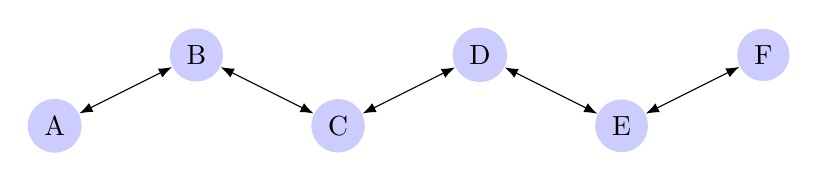
\begin{tikzpicture}  
  [scale=.9,auto=center,every node/.style={circle,fill=blue!20}] 
    
  \node (a1) at (0,0) {A};  
  \node (a2) at (2,1)  {B}; 
  \node (a3) at (4,0)  {C}; 
  \node (a4) at (6,1)  {D}; 
  \node (a5) at (8,0)  {E}; 
  \node (a6) at (10,1)  {F}; 
  
  \path[bidirected] (a1) edge[bend left=0]  (a2); 
  \path[bidirected] (a2) edge[bend left=0]  (a3);
  \path[bidirected] (a4) edge[bend left=0]  (a3);
  \path[bidirected] (a4) edge[bend left=0]  (a5);
  \path[bidirected] (a5) edge[bend left=0]  (a6);
\end{tikzpicture}\\
To check when will a cycle of 6 nodes be created, we assume that there is a chain of 6, in which the start node is Alice and the end node is Frank, with all bidirectional channels. 
\\ Let $U$ be the set of all the nodes. For some node $i$, let $N(i)$ the set of a neighborhood of $i$ within the radius of 1 channel, $L(i)$ be the set of all nodes on the left of $i$, and $R(i)$ be the set of all nodes on the right of $i$. $I_{ij}$ gives the interest return of the payment $c_{ij}$ which is what i sends to j with frequency $\lambda_{ij}$ and is what intermediate nodes save in the channel. 
\\ The interest return and the cost to maintain this network is 
\begin{align}
  I(\lambda) = & \sum_{i\in U}|\sum_{j\in L(i)}\sum_{k\in R(i)\setminus N(i)} I_{jk} - \sum_{j\in R(i)}\sum_{k\in L(i)\setminus N(i)} I_{jk}|\\
  C(\lambda) & = 3(\frac{2B}{r})^{1/3} \sum_{i\in U}|\sum_{j\in L(i)\cup \{i\}}\sum_{k\in R(i)} \lambda_{jk} - \sum_{j\in R(i)}\sum_{k\in L(i)\cup \{i\}} \lambda_{jk}|^{1/3}
  % |\sum_{j\in R(i)\setminus N(i)}I_{ij}(\lambda_{ij})-\sum_{j\in R(i)\setminus N(i)}I_{ji}(\lambda_{ij})|+
  % & + (|\sum_{i\in U}\lambda_{Ai}|^{1/3}+|\sum_{i\in U\setminus\{A\}}\lambda_{Bi}|^{1/3}+|\sum_{i\in \{D,E,F\}}\lambda_{Ci}|^{1/3}\\
  % & +|\sum_{i\in \{E,F\}}\lambda_{Di}|^{1/3}+|\lambda_{EF}|^{1/3})
\end{align}
Note that each term represents the cost for a channel that accounts for intermediate payments; if a frequency is negative, then it counters other directions have allow for rebalancing that makes the channel live longer. 
\\ If Alice build a direct channel with Frank, then each payments has a new route option. 
\\ For example, previously, to send payments to Frank, Alice has the cost to maintain the channel with Bob and all the transaction fees intermediate nodes charge. i.e. Alice's cost to pay Frank without a direct channel is \begin{align}
  C_{ABCDEF} &= T_{BCDE}+ \frac{3}{2}(\frac{2B}{r})^{1/3}(|\sum_{i\in U}\lambda_{Ai}|^{1/3}-|\sum_{i\in U\setminus\{F\}}\lambda_{Ai}|^{1/3})
\end{align}
If Alice choose to create a direct channel with Frank, then she does not need to pay transaction fees, and only pays the cost to maintain that channel.
\\ Thus, She will create the direct channel if 
\begin{align}
  \frac{3}{2}(\frac{2B\lambda_{AF}}{r})^{1/3}\leq &T_{BCDE}+\frac{3}{2}(\frac{2B}{r})^{1/3}(|\sum_{i\in U}\lambda_{Ai}|^{1/3}-|\sum_{i\in U\setminus\{F\}}\lambda_{Ai}|^{1/3})
\end{align}
Note that if Alice created a direct channel with Frank, then it affecs other payments as well,  mainly payments that require transaction fees, as nodes will choose the cheaper route option. 
\\ For example, Bob's payment to Emily: he was paying Emily through CD, but now he can choose to go through AF.
\\ Another example is Alice's payment to Emily, choosing from route BCD and F. 
\begin{align}
  C_{ABCDE} = &T_{BCD}+ \frac{3}{2}(\frac{2B}{r})^{1/3}(|\sum_{i\in U\setminus\{F\}}\lambda_{Ai}|^{1/3}-|\sum_{i\in U\setminus\{E,F\}}\lambda_{Ai}|^{1/3})\\
  C_{AFE} = &T_{F}+ \frac{3}{2}(\frac{2B}{r})^{1/3}(|\lambda_{AD}+\lambda_{AF}|^{1/3}-|\lambda_{AF}|^{1/3})\\
  C_{AE} =& min(C_{ABCDE},C_{AFE})
\end{align}
Inductively, Alice will only consider going through FD to pay Donna if $C_{AE}=C_{AFE}$
\begin{align}
  C_{ABCD} = &T_{BC}+ \frac{3}{2}(\frac{2B}{r})^{1/3}(|\sum_{i\in U\setminus\{F,E\}}\lambda_{Ai}|^{1/3}-|\lambda_{AB}+\lambda_{AC}|^{1/3})\\
  C_{AFED} = &T_{FE}+ \frac{3}{2}(\frac{2B}{r})^{1/3}(|\sum_{i\in U\setminus\{B,C\}}\lambda_{Ai}|^{1/3}-|\lambda_{AF}+\lambda_{AE}|^{1/3})\\
  C_{AD} =& min(C_{ABCD},C_{AFED})
\end{align}
and so on. The same logic applies to other nodes as well, such as Bob paying Frank, Charlie paying Emily. Even though Alice and Frank are the ones that create the channel, if intermediate nodes such as Bob prefers to have an additional route, then they might drive up the transaction fee towards Alice and Frank, forcing them to create a cycle. They might do this when their own transfer payments through other intermediate nodes are too expensive. However, they do not have control over what Alice and Frank charge to go through their channel, so they are still mainly bound by their own creation of a direct channel. 
\\ For Alice, 
\begin{align}
  C_{ABCDEF} =& T_{BCDE}+\frac{3}{2}(\frac{2B}{r})^{1/3}(|\sum_{i\in U}\lambda_{Ai}|^{1/3}-|\sum_{i\in U\setminus\{F\}}\lambda_{Ai}|^{1/3})\\
  C_{AF} =& min(C_{ABCDEF}, \frac{3}{2}(\frac{2B\lambda_{AF}}{r})^{1/3})\\
  C_{ABCDE} = &T_{BCD}+ \frac{3}{2}(\frac{2B}{r})^{1/3}(|\sum_{i\in U\setminus\{F\}}\lambda_{Ai}|^{1/3}-|\sum_{i\in U\setminus\{E,F\}}\lambda_{Ai}|^{1/3})\\
  C_{AFE} = &T_{F}+ \frac{3}{2}(\frac{2B}{r})^{1/3}(|\lambda_{AD}+\lambda_{AF}|^{1/3}-|\lambda_{AF}|^{1/3})\\
  C_{AE} =& min(C_{ABCDE},C_{AFE})\\
  C_{ABCD} = &T_{BC}+ \frac{3}{2}(\frac{2B}{r})^{1/3}(|\sum_{i\in U\setminus\{F,E\}}\lambda_{Ai}|^{1/3}-|\lambda_{AB}+\lambda_{AC}|^{1/3})\\
  C_{AFED} = &T_{FE}+ \frac{3}{2}(\frac{2B}{r})^{1/3}(|\sum_{i\in U\setminus\{B,C\}}\lambda_{Ai}|^{1/3}-|\lambda_{AF}+\lambda_{AE}|^{1/3})\\
  C_{AD} =& min(C_{ABCD},C_{AFED})\\
  C_{ABC} = &T_{B}+ \frac{3}{2}(\frac{2B}{r})^{1/3}(|\lambda_{AB}+\lambda_{AC}|^{1/3}|-|\lambda_{AB}|^{1/3})\\
  C_{AFEDC} = &T_{FED}+ \frac{3}{2}(\frac{2B}{r})^{1/3}(|\sum_{i\in U\setminus\{B\}}\lambda_{Ai}|^{1/3}-|\sum_{i\in U\setminus\{B,C\}}\lambda_{Ai}|^{1/3})\\
  C_{AC} =& min(C_{ABC},C_{AFEDC})\\
  C_{AFEDCB} =& T_{FEDC}+\frac{3}{2}(\frac{2B}{r})^{1/3}(|\sum_{i\in U}\lambda_{Ai}|^{1/3}-|\sum_{i\in U\setminus\{B\}}\lambda_{Ai}|^{1/3})\\
  C_{AB} =& min(C_{AFEDCB}, \frac{3}{2}(\frac{2B\lambda_{AB}}{r})^{1/3})
\end{align}
So when exactly will Alice create a channel with Frank? Assuming that Alice is not expecting to act as an intermedite channel, such that we will not consider the possible transaction fees she can charge, then Alice will create a channel exactly when her cost to pay others is less or equal to if she creates a direct channel. 
\\Together with Frank (with symmetrical reasoning), both of these conditions must be true,
\begin{align}
  \frac{3}{2}(\frac{2B\lambda_{AF}}{r})^{1/3}\leq & \sum_{i\in U} C_{Ai}\\
  \frac{3}{2}(\frac{2B\lambda_{AF}}{r})^{1/3}\leq & \sum_{i\in U} C_{Fi}
\end{align}
Assume that all $\lambda$ is the same, and each node charges the same transaction fee.
\begin{align}
  C_{ABCDEF} =& 4T+\frac{3}{2}(\frac{2B}{r})^{1/3}(|5\lambda|^{1/3}-|4\lambda|^{1/3})\\
  C_{AF} =& min(C_{ABCDEF}, \frac{3}{2}(\frac{2B\lambda}{r})^{1/3})\\
  C_{ABCDE} = &3T+ \frac{3}{2}(\frac{2B}{r})^{1/3}(|4\lambda|^{1/3}-|3\lambda|^{1/3})\\
  C_{AFE} = &T+ \frac{3}{2}(\frac{2B}{r})^{1/3}(|2\lambda|^{1/3}-|\lambda|^{1/3})\\
  C_{AE} =& min(C_{ABCDE},C_{AFE})\\
  C_{ABCD} = &2T+ \frac{3}{2}(\frac{2B}{r})^{1/3}(|3\lambda|^{1/3}-|2\lambda|^{1/3})\\
  C_{AFED} = &2T+ \frac{3}{2}(\frac{2B}{r})^{1/3}(|3\lambda|^{1/3}-|2\lambda|^{1/3})\\
  C_{AD} =& min(C_{ABCD},C_{AFED})\\
  C_{ABC} = &T+ \frac{3}{2}(\frac{2B}{r})^{1/3}(|2\lambda|^{1/3}|-|\lambda|^{1/3})\\
  C_{AFEDC} = &3T+ \frac{3}{2}(\frac{2B}{r})^{1/3}(|4\lambda|^{1/3}-|3\lambda|^{1/3})\\
  C_{AC} =& min(C_{ABC},C_{AFEDC})\\
  C_{AFEDCB} =& 4T+\frac{3}{2}(\frac{2B}{r})^{1/3}(|5\lambda|^{1/3}-|4\lambda|^{1/3})\\
  C_{AB} =& min(C_{AFEDCB}, \frac{3}{2}(\frac{2B\lambda}{r})^{1/3})
\end{align}
Analyze each payments, assume that $\lambda>0$ and $T\geq 0$
\begin{align}
  C_{ABCDEF} =& 4T+\frac{3}{2}(\frac{2B}{r})^{1/3}(|5\lambda|^{1/3}-|4\lambda|^{1/3}) = 4T+\frac{3}{2}(\frac{2B\lambda}{r})^{1/3}(5^{1/3}-4^{1/3})\\
  C_{AF} =& min(4T+\frac{3}{2}(\frac{2B\lambda}{r})^{1/3}(5^{1/3}-4^{1/3}), \frac{3}{2}(\frac{2B\lambda}{r})^{1/3})\\
  =&min(4T+\frac{3}{2}(\frac{2B\lambda}{r})^{1/3}(.122575), \frac{3}{2}(\frac{2B\lambda}{r})^{1/3})\\
  C_{AF} &=\frac{3}{2}(\frac{2B\lambda}{r})^{1/3}  \iff T(\frac{r}{B\lambda})^{1/3} \geq .4146\\
  C_{AF} &=4T+\frac{3}{2}(\frac{2B\lambda}{r})^{1/3}(.122575) \iff T(\frac{r}{B\lambda})^{1/3} \leq .4146
\end{align}
Assume that $T(\frac{r}{B\lambda})^{1/3} \geq .4146$, such that the direct channel is better than routing through BCDE, so we continus with the next payment
\begin{align}
  C_{ABCDE} &= 3T+ \frac{3}{2}(\frac{2B\lambda}{r})^{1/3}(4^{1/3}-3^{1/3})\\
  C_{AFE} &= T+ \frac{3}{2}(\frac{2B\lambda}{r})^{1/3}(2^{1/3}-1)\\
  C_{AE} &= min(C_{ABCDE},C_{AFE}) = C_{ABCDE} 
  % \\ \iff & T\leq (\frac{B\lambda}{r})^{1/3}(.1085)
  \\ \iff & T (\frac{r}{B\lambda})^{1/3} \leq .1085\\
  C_{AE} &= min(C_{ABCDE},C_{AFE}) = C_{AFE} \\
  % \iff & 2T+ \frac{3}{2}(\frac{2B\lambda}{r})^{1/3}(4^{1/3}-3^{1/3}) \geq \frac{3}{2}(\frac{2B\lambda}{r})^{1/3}(2^{1/3}-1)\\ 
  \iff & T (\frac{r}{B\lambda})^{1/3} \geq .1085
\end{align}
Since $T(\frac{r}{B\lambda})^{1/3} \geq .4146 > .1085$, then F is the better route than BCD, we analyze the next payment
\begin{align}
  C_{ABCD} = &2T+ \frac{3}{2}(\frac{2B}{r})^{1/3}(|3\lambda|^{1/3}-|2\lambda|^{1/3})\\
  C_{AFED} = &2T+ \frac{3}{2}(\frac{2B}{r})^{1/3}(|3\lambda|^{1/3}-|2\lambda|^{1/3})\\
  C_{AD} =& min(C_{ABCD},C_{AFED}) = C_{ABCD}=C_{AFED}
\end{align}
This means that either route costs the same. Assume that Alice choose to go through the FE route, let's go further into analyzing the payments.
\begin{align}
  C_{ABC} = &T+ \frac{3}{2}(\frac{2B}{r})^{1/3}(|2\lambda|^{1/3}|-|\lambda|^{1/3})\\
  C_{AFEDC} = &3T+ \frac{3}{2}(\frac{2B}{r})^{1/3}(|4\lambda|^{1/3}-|3\lambda|^{1/3})\\
  C_{AC} =& min(C_{ABC},C_{AFEDC})\\
  C_{AC} = C_{ABC} \iff & \frac{3}{2}(\frac{2B}{r})^{1/3}(|2\lambda|^{1/3}|-|\lambda|^{1/3}) \leq 2T+ \frac{3}{2}(\frac{2B}{r})^{1/3}(|4\lambda|^{1/3}-|3\lambda|^{1/3})\\
  \iff & T (\frac{r}{B\lambda})^{1/3} \geq .1085 \\
  C_{AC} = C_{AFEDC} \iff & T (\frac{r}{B\lambda})^{1/3} \leq .1085
  % C_{AFEDCB} =& 4T+\frac{3}{2}(\frac{2B}{r})^{1/3}(|5\lambda|^{1/3}-|4\lambda|^{1/3})\\
  % C_{AB} =& min(C_{AFEDCB}, \frac{3}{2}(\frac{2B\lambda}{r})^{1/3})
\end{align}
Since we assumed that $T (\frac{r}{B\lambda})^{1/3} \geq .1085$ when we are choosing between F and BCD,, this means that route FED cannot be better than route B when Alice wants to pay Charlie. Hence, Alice chooses the route B. Inductively, Alice uses the direct channel to pay Bob.
\\ In conclusion, Alice will send payments to both directions, and the direction she chooses depends on the length of the route when other parameters are held constant and equal. The only necessary condition for Alice to create a direct channel with Frank is if $T(\frac{r}{B\lambda})^{1/3} \geq .4146$. 
\\ What happens if $.4146 \geq T(\frac{r}{B\lambda})^{1/3} \geq .1085$?
\\ What happens to the network's global benefits when will $T (\frac{r}{B\lambda})^{1/3} \geq .4146$? 












\subsection{if $.4146 (\frac{B\lambda}{r})^{1/3} \geq T \geq .1085 (\frac{B\lambda}{r})^{1/3} $}
\begin{align}
  .665652 (\frac{B\lambda}{r})^{1/3} & \leq C_{ABCDEF} \leq  1.8900 (\frac{B\lambda}{r})^{1/3})\\
  C_{AF} =& min(C_{ABCDEF}, 1.8900(\frac{B\lambda}{r})^{1/3})=1.8900(\frac{B\lambda}{r})^{1/3}\\
  C_{ABCDE} = &3T+ \frac{3}{2}(\frac{2B}{r})^{1/3}(|4\lambda|^{1/3}-|3\lambda|^{1/3})\\
  C_{AFE} = &T+ \frac{3}{2}(\frac{2B}{r})^{1/3}(|2\lambda|^{1/3}-|\lambda|^{1/3})\\
  C_{AE} =& min(C_{ABCDE},C_{AFE})=min(2T+ .2743(\frac{B\lambda}{r})^{1/3}, .49122(\frac{B\lambda}{r})^{1/3})\\
  & \geq min(.4912(\frac{B\lambda}{r})^{1/3}, .4912(\frac{B\lambda}{r})^{1/3})=C_{AFE}\\
  C_{ABCD} = &2T+ \frac{3}{2}(\frac{2B}{r})^{1/3}(|3\lambda|^{1/3}-|2\lambda|^{1/3})\\
  C_{AFED} = &2T+ \frac{3}{2}(\frac{2B}{r})^{1/3}(|3\lambda|^{1/3}-|2\lambda|^{1/3})\\
  C_{AD} =& min(C_{ABCD},C_{AFED})\\
  C_{ABC} = &T+ \frac{3}{2}(\frac{2B}{r})^{1/3}(|2\lambda|^{1/3}|-|\lambda|^{1/3})\\
  C_{AFEDC} = &3T+ \frac{3}{2}(\frac{2B}{r})^{1/3}(|4\lambda|^{1/3}-|3\lambda|^{1/3})\\
  C_{AC} =& min(C_{ABC},C_{AFEDC})\\
  C_{AFEDCB} =& 4T+\frac{3}{2}(\frac{2B}{r})^{1/3}(|5\lambda|^{1/3}-|4\lambda|^{1/3})\\
  C_{AB} =& min(C_{AFEDCB}, \frac{3}{2}(\frac{2B\lambda}{r})^{1/3})
\end{align}















\subsection{Global benefit}
Recall that the interest return and the cost to maintain the network are
\begin{align}
  I(\lambda) = & \sum_{i\in U}|\sum_{j\in L(i)}\sum_{k\in R(i)\setminus N(i)} I_{jk} - \sum_{j\in R(i)}\sum_{k\in L(i)\setminus N(i)} I_{jk}|\\
  C(\lambda) & = 3(\frac{2B}{r})^{1/3} \sum_{i\in U}|\sum_{j\in L(i)\cup \{i\}}\sum_{k\in R(i)} \lambda_{jk} - \sum_{j\in R(i)}\sum_{k\in L(i)\cup \{i\}} \lambda_{jk}|^{1/3}
\end{align}
Let all $\lambda$ and $I$ be the same, then 
\begin{align}
  I(\lambda) = & \sum_{i\in U}|\sum_{j\in L(i)}\sum_{k\in R(i)\setminus N(i)} I_{jk} - \sum_{j\in R(i)}\sum_{k\in L(i)\setminus N(i)} I_{jk}|\\
  C(\lambda) & = 3(\frac{2B}{r})^{1/3} \sum_{i\in U}|\sum_{j\in L(i)\cup \{i\}}\sum_{k\in R(i)} \lambda_{jk} - \sum_{j\in R(i)}\sum_{k\in L(i)\cup \{i\}} \lambda_{jk}|^{1/3}
\end{align}
Let's build a matrix of the payments\\ $
\begin{matrix}
  sender\backslash receive & A & B & C & D & E & F\\
  A & 0 & c_{AB} & c_{AC} & c_{AD} & c_{AE} & c_{AF}
\end{matrix}
$
% When will it be beneficial to have a 6 nodes cycle? We analyze the benefits by comparing it with other structures with 6 nodes. For simplicity, let all the channel be bidirectional. Let $d_n$ be degree of n for $n=A,B,...,F$
% \begin{enumerate}
%     \item $A\rightleftarrows B \rightleftarrows C \rightleftarrows D \rightleftarrows E \rightleftarrows F$ (a chain, $d_n\leq 2$)
%     \item $A\rightleftarrows B \rightleftarrows C \rightleftarrows D$, $B \rightleftarrows E \rightleftarrows F$ (fork with subfork length 2, $d_n\leq 3$)
%     \item $A\rightleftarrows B \rightleftarrows C \rightleftarrows D \rightleftarrows E $, $D \rightleftarrows F$ (fork with subfork length 1, $d_n\leq 3$)
%     \item $(A,E)\rightleftarrows B \rightleftarrows C \rightleftarrows (D,F) $ (2 fork with connected parents. Subfork length 1, $d_n\leq 3$)
%     \item $A\rightleftarrows B \rightleftarrows C \rightleftarrows (D,E,F)$ (tri-fork with subfork length 1, $d_n\leq 4$)
%     \item $A\rightleftarrows (B,C,D,E,F)$ (5-sided web with subfork length 1, $d_n\leq 4$)
%     \item $A\rightleftarrows B \rightleftarrows C \rightleftarrows D \rightleftarrows E \rightleftarrows F \rightleftarrows A$ (a cycle, $d_n\leq 2$)
% \end{enumerate}
% First we analyze the total cost to maintain the structures. Let each of the frequencies be $\lambda_{ij}=-\lambda_{ji}$, for simplicity of the notations, assume each of the following used the positive frequency regardless of the indicated direction, i.e. $AF \sim FA$
% \\ Need to come up with some notation that represent all the possible transactions between all the nodes from A to F. Aside from structure 7, removing an edge will lead of disconnected components. Let $(U,V)$ be the sets that contains the nodes from the 2 disconnected components if we ignore the channel $uv$. Let $\lambda_{uv}=|\sum_{v' \in V}\lambda_{uv'}-\sum_{u'\in U} \lambda_{u'v}|$, and $I_{uv}=max_{u'\in U\setminus\{u\}}(I_{u'v})+max_{v'\in V\setminus\{v\}}(I_{uv'})$
% \begin{align}
%     C_{S1} & = 3(\frac{2B}{r})^{1/3}((\lambda_{AB})^{1/3}+(\lambda_{BC})^{1/3}+(\lambda_{CD})^{1/3} +(\lambda_{DE})^{1/3}+(\lambda_{EF})^{1/3})\\
%     C_{S2} & = 2I_{AF} + 3(\frac{2B}{r})^{1/3}((\lambda_{AB})^{1/3}+\lambda_{BC}^{1/3}+\lambda_{CD}^{1/3}+(\lambda_{BE})^{1/3}\\
%     & +(\lambda_{EF})^{1/3})\\
%     C_{S3} & = 3I_{AF} + 3(\frac{2B}{r})^{1/3}((\lambda_{AB})^{1/3}+(\lambda_{BC})^{1/3}+(\lambda_{CD})^{1/3}+\lambda_{DE}^{1/3}\\
%     & +(\lambda_{DF}+\lambda_{FA})^{1/3})\\
%     C_{S4} & = 2I_{AF} + 3(\frac{2B}{r})^{1/3}((\lambda_{AB}+\lambda_{FA})^{1/3}+(\lambda_{BC}+\lambda_{FA})^{1/3}+\lambda_{CD}^{1/3}+\lambda_{BE}^{1/3}\\
%     & +(\lambda_{CF}+\lambda_{FA})^{1/3})\\
%     C_{S5} & = 2I_{AF}+3(\frac{2B}{r})^{1/3}((\lambda_{AB}+\lambda_{FA})^{1/3}+(\lambda_{BC}+\lambda_{FA})^{1/3}+\lambda_{CD}^{1/3}+\lambda_{CE}^{1/3}\\
%     & +(\lambda_{CF}+\lambda_{FA})^{1/3})\\
%     C_{S6} & = 3(\frac{2B}{r})^{1/3}(\lambda_{AB}^{1/3}+\lambda_{AC}^{1/3}+\lambda_{AD}^{1/3}+\lambda_{AE}^{1/3}+\lambda_{AF}^{1/3})\\
%     C_{S7} & = 3(\frac{2B}{r})^{1/3}(\lambda_{AB}^{1/3}+\lambda_{BC}^{1/3}+\lambda_{CD}^{1/3}+\lambda_{DE}^{1/3}+\lambda_{EF}^{1/3}+\lambda_{FA}^{1/3})
% \end{align}
% Note that if there is no transactions between Alice and Frank, secifically $\lambda_{AF}=0$ and $I_{AF}=0$, and if all other frequencies are equal, then all the cost of maintainence is the same. 
% Note that $C_{S1}\leq C_{S7}$, and if the frequencies are equal, then $C_{S7}$ is a more expensive structure to maintain. We then evaluate the costs with transative nodes and try to find when $C'_{S7}$ is beneficial. For all these cases, we do not allow new channels. 
% \begin{enumerate}
%     \item Alice sends transactions to Charlie. We analyze the change in structures 1, 6, and 7. 
%     \item Alice sends transactions to Donna. Analyze the change in structures 1 and 7.
%     \item Alice sends transactions to Emily. Analyze structures 1 and 7.
%     \item Alice sends transactions to Frank. Analyze structures 1 and 7.
%     \item Bob sends transactions to Charlie. Analyze structures 6 and 7.
%     \item Bob sends transactions to Donna. Analyze structures 2, 
%     \item ...
% \end{enumerate}
% \subsubsection{Case 1}
% Alice sends transactions to Charlie. We analyze the change in structures 1, 6, and 7. 
% \\ The new costs to maintaining each structures, including opportunity cost $I_{AC}$ for each intermediate node
% % \begin{align}
% %     C_{S1} & = 4I_{AF}+ I_{AC} +3(\frac{2B}{r})^{1/3}((\lambda_{AB}+\lambda_{FA}+\lambda_{AC})^{1/3}+(\lambda_{BC}+\lambda_{FA}+\lambda_{AC})^{1/3}\\ 
% %     & +(\lambda_{CD}+\lambda_{FA})^{1/3}+(\lambda_{DE}+\lambda_{FA})^{1/3}+(\lambda_{EF}+\lambda_{FA})^{1/3})\\
% %     C_{S6} & = 3(\frac{2B}{r})^{1/3}(\lambda_{AB}^{1/3}+\lambda_{AC}^{1/3}+\lambda_{AD}^{1/3}+\lambda_{AE}^{1/3}+\lambda_{AF}^{1/3})\\
% %     C_{S7_1} & = I_{AC} + 3(\frac{2B}{r})^{1/3}((\lambda_{AB}+\lambda_{AC})^{1/3}+(\lambda_{BC}+\lambda_{AC})^{1/3}+\lambda_{CD}^{1/3}+\lambda_{DE}^{1/3}+\lambda_{EF}^{1/3}\\
% %     & +\lambda_{FA}^{1/3})\\
% %     C_{S7_2} & = 3I_{AC} + 3(\frac{2B}{r})^{1/3}(\lambda_{AB}^{1/3}+\lambda_{BC}^{1/3}+(\lambda_{CD}+\lambda_{AC})^{1/3}+(\lambda_{DE}+\lambda_{AC})^{1/3}\\
% %     & +(\lambda_{EF}+\lambda_{AC})^{1/3}+ (\lambda_{FA}+\lambda_{AC})^{1/3})
% % \end{align}
% % Where
% % \begin{align}
% %     C_{S7_1}& \leq C_{S1} \iff (\lambda_{AB}+\lambda_{AC})^{1/3}+(\lambda_{BC}+\lambda_{AC})^{1/3}+\lambda_{CD}^{1/3}+\lambda_{DE}^{1/3}+\lambda_{EF}^{1/3} +\lambda_{FA}^{1/3}  \\
% %     \leq & \frac{4I_{AF}r^{1/3}}{3(2B)^{1/3}}+ (\lambda_{AB}+\lambda_{FA}+\lambda_{AC})^{1/3}+(\lambda_{BC}+\lambda_{FA}+\lambda_{AC})^{1/3}+(\lambda_{CD}+\lambda_{FA})^{1/3}\\ 
% %     & +(\lambda_{DE}+\lambda_{FA})^{1/3}+(\lambda_{EF}+\lambda_{FA})^{1/3}
% % \end{align}
% % Note that they are equivalent if $\lambda_{FA}=0$ and $I_{AF}=0$
% % \\ Also, 
% % \begin{align}
% %     C_{S7_2}& \leq C_{S1} \iff \frac{2I_{AC}r^{1/3}}{3(2B)^{1/3}} + \lambda_{AB}^{1/3}+\lambda_{BC}^{1/3}+(\lambda_{CD}+\lambda_{AC})^{1/3}+(\lambda_{DE}+\lambda_{AC})^{1/3}\\
% %     & +(\lambda_{EF}+\lambda_{AC})^{1/3}+ (\lambda_{FA}+\lambda_{AC})^{1/3}\\
% %     \leq & \frac{4I_{AF}r^{1/3}}{3(2B)^{1/3}}+(\lambda_{AB}+\lambda_{FA}+\lambda_{AC})^{1/3}+(\lambda_{BC}+\lambda_{FA}+\lambda_{AC})^{1/3}+(\lambda_{CD}+\lambda_{FA})^{1/3}\\ 
% %     & +(\lambda_{DE}+\lambda_{FA})^{1/3}+(\lambda_{EF}+\lambda_{FA})^{1/3}
% % \end{align}
% % There are cases in which the route with longer length provides a lower cost of maintainence. 

% % \subsubsection{Case 2}
% % Alice sends transactions to Donna. Analyze the change in structures 1 and 7.
% % \begin{align}
% %     C_{S1} & = 2I_{AC} + 3(\frac{2B}{r})^{1/3}((\lambda_{AB}+\lambda_{AC})^{1/3}\\
% %     &+(\lambda_{BC}+\lambda_{AC})^{1/3}+(\lambda_{CD}+\lambda_{AC})^{1/3}+\lambda_{DE}^{1/3}+\lambda_{EF}^{1/3})\\
% %     C_{S7_1} & = 2I_{AC}+3(\frac{2B}{r})^{1/3}((\lambda_{AB}+\lambda_{AC})^{1/3}\\
% %     & +(\lambda_{BC}+\lambda_{AC})^{1/3}+(\lambda_{CD}+\lambda_{AC})^{1/3}+\lambda_{DE}^{1/3}+\lambda_{EF}^{1/3}+ \lambda_{FA}^{1/3})\\
% %     C_{S7_2} & = 2I_{AC} + 3(\frac{2B}{r})^{1/3}(\lambda_{AB}^{1/3}+\lambda_{BC}^{1/3}\\
% %     & +\lambda_{CD}^{1/3}+(\lambda_{DE}+\lambda_{AC})^{1/3}+(\lambda_{EF}+\lambda_{AC})^{1/3}+ (\lambda_{FA}+\lambda_{AC})^{1/3})
% % \end{align}

% % \begin{align}
% %     C_{S1} & = 2I_{AD}+4I_{AF}+3(\frac{2B}{r})^{1/3}((\lambda_{AB}+\lambda_{FA}+\lambda_{AD})^{1/3}+(\lambda_{BC}+\lambda_{FA}+\lambda_{AD})^{1/3}+(\lambda_{CD}+\lambda_{FA}+\lambda_{AD})^{1/3}\\ 
% %     & +(\lambda_{DE}+\lambda_{FA})^{1/3}+(\lambda_{EF}+\lambda_{FA})^{1/3})\\
% %     C_{S2} & = 2I_{AD}+2I_{AF} + 3(\frac{2B}{r})^{1/3}((\lambda_{AB}+\lambda_{FA}+\lambda_{AD})^{1/3}+(\lambda_{BC}+\lambda_{AD})^{1/3}+(\lambda_{CD}+\lambda_{AD})^{1/3}+(\lambda_{BE}+\lambda_{FA})^{1/3}\\
% %     & +(\lambda_{EF}+\lambda_{FA})^{1/3})\\
% %     C_{S4} & = 2I_{AD}+ 2I_{AF} + 3(\frac{2B}{r})^{1/3}((\lambda_{AB}+\lambda_{FA}+\lambda_{AD})^{1/3}+(\lambda_{BC}+\lambda_{FA}+\lambda_{AD})^{1/3}+(\lambda_{CD}+\lambda_{AD})^{1/3}+\lambda_{BE}^{1/3}\\
% %     & +(\lambda_{CF}+\lambda_{FA})^{1/3})\\
% %     C_{S6} & = 3(\frac{2B}{r})^{1/3}(\lambda_{AB}^{1/3}+\lambda_{AC}^{1/3}+\lambda_{AD}^{1/3}+\lambda_{AE}^{1/3}+\lambda_{AF}^{1/3})\\
% %     C_{S7} & = 3(\frac{2B}{r})^{1/3}(\lambda_{AB}^{1/3}+\lambda_{BC}^{1/3}+\lambda_{CD}^{1/3}+\lambda_{DE}^{1/3}+\lambda_{EF}^{1/3}+\lambda_{FA}^{1/3})
% % \end{align}
% % For $C_{S7_2}\leq C_{S1}$, 
% % \begin{align}
% %     & \lambda_{AB}^{1/3}+\lambda_{BC}^{1/3}+\lambda_{CD}^{1/3}+(\lambda_{DE}+\lambda_{AC})^{1/3}+(\lambda_{EF}+\lambda_{AC})^{1/3}+ (\lambda_{FA}+\lambda_{AC})^{1/3}\\
% %     \leq & (\lambda_{AB}+\lambda_{AC})^{1/3}+(\lambda_{BC}+\lambda_{AC})^{1/3}+(\lambda_{CD}+\lambda_{AC})^{1/3}+\lambda_{DE}^{1/3}+\lambda_{EF}^{1/3}
% % \end{align}


% % \subsubsection{Case 3}
% % Alice sends transactions to Emily. Analyze the change in structures 1 and 7.
% % \begin{align}
% %     C_{S1} & = 3I_{AC} + 3(\frac{2B}{r})^{1/3}((\lambda_{AB}+\lambda_{AC})^{1/3}\\
% %     &+(\lambda_{BC}+\lambda_{AC})^{1/3}+(\lambda_{CD}+\lambda_{AC})^{1/3}+(\lambda_{DE}+\lambda_{AC})^{1/3}+\lambda_{EF}^{1/3})\\
% %     C_{S7_2} & = 2I_{AC} + 3(\frac{2B}{r})^{1/3}(\lambda_{AB}^{1/3}+\lambda_{BC}^{1/3}\\
% %     & +\lambda_{CD}^{1/3}+\lambda_{DE}^{1/3}+(\lambda_{EF}+\lambda_{AC})^{1/3}+ (\lambda_{FA}+\lambda_{AC})^{1/3})
% % \end{align}

% % \subsubsection{Case 4}
% % Alice sends transactions to Frank. Analyze the change in structures 1 and 7.
% % \begin{align}
% %     C_{S1} & = 4I_{AC} + 3(\frac{2B}{r})^{1/3}((\lambda_{AB}+\lambda_{AC})^{1/3}\\
% %     &+(\lambda_{BC}+\lambda_{AC})^{1/3}+(\lambda_{CD}+\lambda_{AC})^{1/3}+\lambda_{DE}^{1/3}+(\lambda_{EF}+\lambda_{AC})^{1/3})\\
% %     C_{S7_2} & = 2I_{AC} + 3(\frac{2B}{r})^{1/3}(\lambda_{AB}^{1/3}+\lambda_{BC}^{1/3}+\lambda_{CD}^{1/3}+\lambda_{DE}^{1/3}+\lambda_{EF}^{1/3}+ \lambda_{FA}^{1/3})
% % \end{align}
% % For $C_{S7_2}\leq C_{S1}$, 
% % \begin{align}
% %     & \lambda_{AB}^{1/3}+\lambda_{BC}^{1/3}+\lambda_{CD}^{1/3}+(\lambda_{DE}+\lambda_{AC})^{1/3}+(\lambda_{EF}+\lambda_{AC})^{1/3}+ (\lambda_{FA}+\lambda_{AC})^{1/3}\\
% %     \leq & (\lambda_{AB}+\lambda_{AC})^{1/3}+(\lambda_{BC}+\lambda_{AC})^{1/3}+(\lambda_{CD}+\lambda_{AC})^{1/3}+\lambda_{DE}^{1/3}+\lambda_{EF}^{1/3}
% % \end{align}


\newpage
new page
\end{document}

%   T &\geq I(c)+C_{n}-C_{o}
%   T &\leq C_{o} - C_{n}
%   T &= \frac{p\lambda}{mr}\cdot c
%   I &= \frac{m\alpha}{r}-m



% \begin{align}
%     C_{S1} & = 4I_{AF}+3(\frac{2B}{r})^{1/3}((\lambda_{AB}+\lambda_{FA})^{1/3}+(\lambda_{BC}+\lambda_{FA})^{1/3}+(\lambda_{CD}+\lambda_{FA})^{1/3}\\ 
%     & +(\lambda_{DE}+\lambda_{FA})^{1/3}+(\lambda_{EF}+\lambda_{FA})^{1/3})\\
%     C_{S2} & = 2I_{AF} + 3(\frac{2B}{r})^{1/3}((\lambda_{AB}+\lambda_{FA})^{1/3}+\lambda_{BC}^{1/3}+\lambda_{CD}^{1/3}+(\lambda_{BE}+\lambda_{FA})^{1/3}\\
%     & +(\lambda_{EF}+\lambda_{FA})^{1/3})\\
%     C_{S3} & = 3I_{AF} + 3(\frac{2B}{r})^{1/3}((\lambda_{AB}+\lambda_{FA})^{1/3}+(\lambda_{BC}+\lambda_{FA})^{1/3}+(\lambda_{CD}+\lambda_{FA})^{1/3}+\lambda_{DE}^{1/3}\\
%     & +(\lambda_{DF}+\lambda_{FA})^{1/3})\\
%     C_{S4} & = 2I_{AF} + 3(\frac{2B}{r})^{1/3}((\lambda_{AB}+\lambda_{FA})^{1/3}+(\lambda_{BC}+\lambda_{FA})^{1/3}+\lambda_{CD}^{1/3}+\lambda_{BE}^{1/3}\\
%     & +(\lambda_{CF}+\lambda_{FA})^{1/3})\\
%     C_{S5} & = 2I_{AF}+3(\frac{2B}{r})^{1/3}((\lambda_{AB}+\lambda_{FA})^{1/3}+(\lambda_{BC}+\lambda_{FA})^{1/3}+\lambda_{CD}^{1/3}+\lambda_{CE}^{1/3}\\
%     & +(\lambda_{CF}+\lambda_{FA})^{1/3})\\
%     C_{S6} & = 3(\frac{2B}{r})^{1/3}(\lambda_{AB}^{1/3}+\lambda_{AC}^{1/3}+\lambda_{AD}^{1/3}+\lambda_{AE}^{1/3}+\lambda_{AF}^{1/3})\\
%     C_{S7} & = 3(\frac{2B}{r})^{1/3}(\lambda_{AB}^{1/3}+\lambda_{BC}^{1/3}+\lambda_{CD}^{1/3}+\lambda_{DE}^{1/3}+\lambda_{EF}^{1/3}+\lambda_{FA}^{1/3})
% \end{align}